\section{Tests Environment and Results}

The previous section described how the system was implemented and how each component interacts within the complete flow — from a user uploading a file to the leader performing the corruption check in the Raft cluster.

This section presents the testing environment, the scenarios used during evaluation, and the obtained results. The tests were executed on a cluster of nine machines running Ubuntu 24.04.1 LTS (GNU/Linux 6.8.0-51-generic x86\_64). The specifications of the virtual machines are summarized in Table \ref{tab:vms-specs}. The nodes were geographically distributed across the European continent.

\begin{table}[h!]
    \centering
    \begin{tabular}{|l|c|c|c|c|}
    \hline
       \textbf{Node ID} & \textbf{IPv4} & \textbf{CPU(s)} & \textbf{RAM} & \textbf{Disk} \\
       \hline
        GW & 51.15.221.121 & 8 & 32 GB & 45 GB \\
        Agent 1 & 212.47.241.22 & 4 & 16 GB & 45 GB \\
        Agent 2 & 51.15.138.169 & 4 & 16 GB & 45 GB \\
        Agent 3 & 51.159.178.75 & 4 & 8 GB & 45 GB \\
        Agent 4 & 51.158.75.32 & 4 & 8 GB & 45 GB \\
        Agent 5 & 51.158.233.202 & 4 & 8 GB & 45 GB \\
        Agent 6 & 51.15.108.2 & 4 & 8 GB & 45 GB \\
        Agent 7 & 151.115.42.176 & 4 & 8 GB & 45 GB \\
        Agent 8 & 151.115.104.48 & 4 & 8 GB & 45 GB \\
        \hline
    \end{tabular}
    \caption{Specifications of the machines used in the testing environment.}
    \label{tab:vms-specs}
\end{table}

Each test scenario considered four parameters:
\begin{itemize}
    \item \textbf{Number of agents}: total number of agents participating in the Reed–Solomon configuration of $n + k$ nodes.
    \item \textbf{Number of offline agents}: number of agents intentionally disconnected during the Corruption Check phase.
    \item \textbf{Number of files}: number of files included in the test.
    \item \textbf{File size}: size of each uploaded file. Since each file is divided into $n + k$ shards, the size of a single shard equals $\frac{\text{file size}}{\text{number of agents}}$ bytes.
\end{itemize}

After each upload, the environment was tested through the Corruption Check phase, measuring the total elapsed time in seconds from the initial check request to its completion. Each plot reports the average total elapsed time over three independent runs.

\paragraph{Test 1}
In this first scenario, we uploaded 100 files, each 100~MB in size, for a total dataset of 10~GB. Each file was divided into $n + k$ shards and distributed across the agents in the cluster. All agents remained online during the Corruption Check phase. Figure~\ref{fig:test-1} illustrates the elapsed time for the corruption check as the number of agents varies from 3 to 8. As expected, the elapsed time increases with the number of agents due to the greater number of shard verifications required.

\begin{figure}[!ht]
\centering
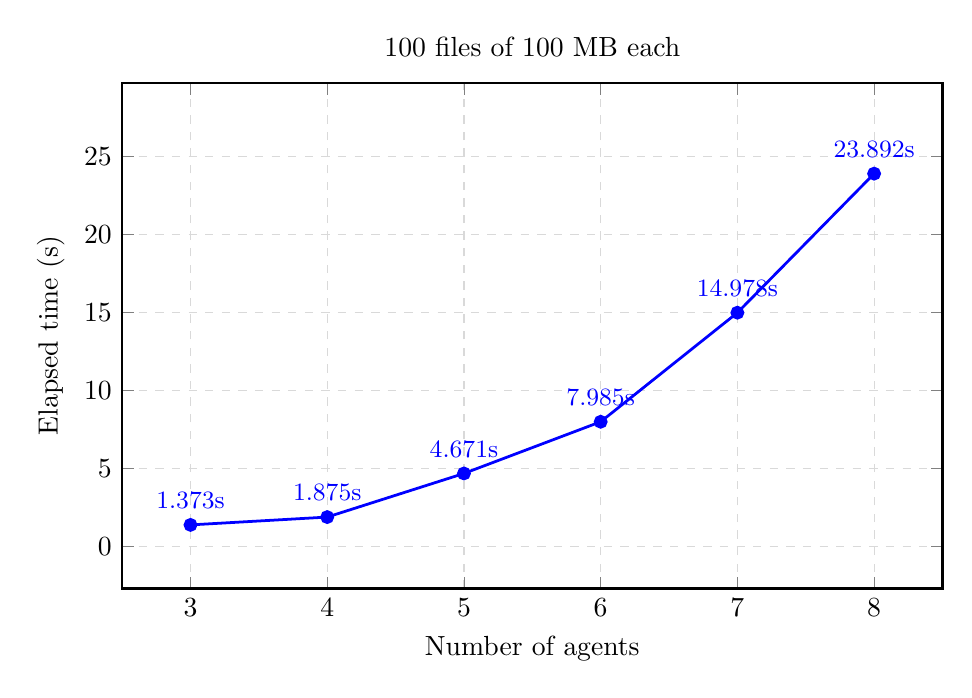
\begin{tikzpicture}
\begin{axis}[
    width=12cm, height=8cm,
    xlabel={Number of agents},
    ylabel={Elapsed time (s)},
    xmin=3, xmax=8,
    ymin=0, ymax=27,
    xtick={3,4,5,6,7,8},
    ytick={0,5,10,15,20,25},
    grid=major,
    grid style={dashed,gray!30},
    thick,
    title={100 files of 100~MB each},
    enlargelimits=0.1,
    clip=false,
    nodes near coords,
    every node near coord/.append style={font=\small, anchor=south, yshift=2pt},
    point meta=explicit symbolic
]

\addplot[color=blue, mark=*, line width=1pt] coordinates {
    (3,1.373) [1.373s]
    (4,1.875) [1.875s]
    (5,4.671) [4.671s]
    (6,7.985) [7.985s]
    (7,14.978) [14.978s]
    (8,23.892) [23.892s]
};
\end{axis}
\end{tikzpicture}
\caption{Elapsed time of the Corruption Check phase with 0 offline agents.}
\label{fig:test-1}
\end{figure}

\newpage
\paragraph{Test 2}
In the second test, we uploaded 10,000 files of 1~MB each, maintaining the same total dataset size of 10~GB as in Test 1. This scenario highlights the effect of having many small files instead of fewer large files. All agents remained online. As shown in Figure~\ref{fig:test-2}, the elapsed time grows significantly as the number of agents increases, reflecting the overhead of managing and verifying a large number of small shards.

\begin{figure}[!ht]
\centering
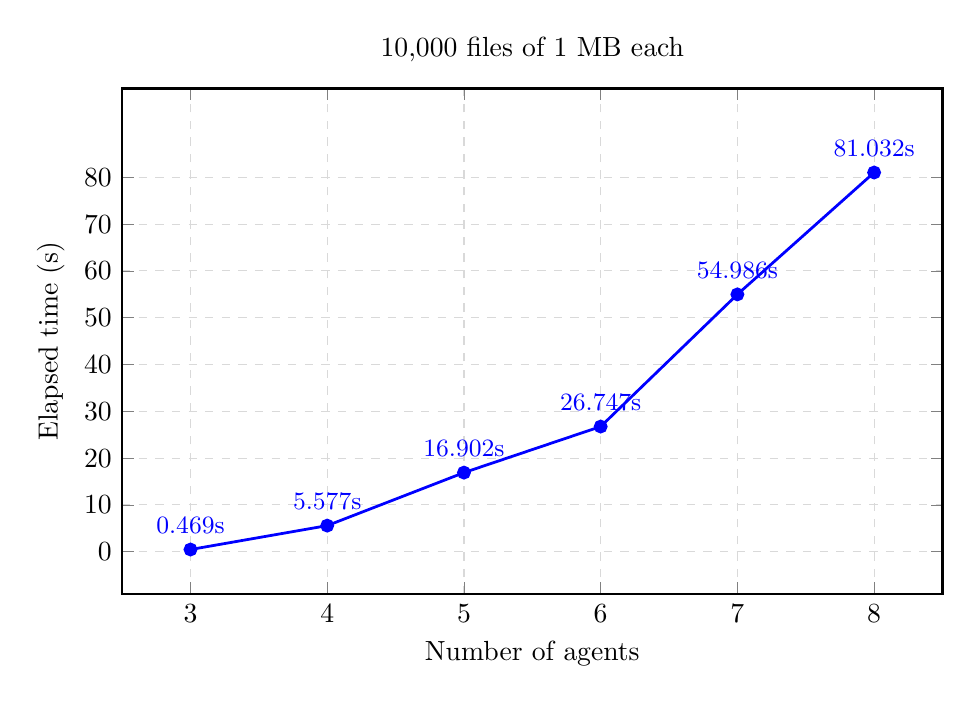
\begin{tikzpicture}
\begin{axis}[
    width=12cm, height=8cm,
    xlabel={Number of agents},
    ylabel={Elapsed time (s)},
    xmin=3, xmax=8,
    ymin=0, ymax=90,
    xtick={3,4,5,6,7,8},
    ytick={0,10,20,30,40,50,60,70,80},
    grid=major,
    grid style={dashed,gray!30},
    thick,
    title={10,000 files of 1~MB each},
    enlargelimits=0.1,
    clip=false,
    nodes near coords,
    every node near coord/.append style={font=\small, anchor=south, yshift=2pt},
    point meta=explicit symbolic
]

\addplot[color=blue, mark=*, line width=1pt] coordinates {
    (3,0.4685) [0.469s]
    (4,5.577) [5.577s]
    (5,16.902) [16.902s]
    (6,26.747) [26.747s]
    (7,54.986) [54.986s]
    (8,81.032) [81.032s]
};
\end{axis}
\end{tikzpicture}
\caption{Elapsed time of the Corruption Check phase with 0 offline agents.}
\label{fig:test-2}
\end{figure}

\newpage
\paragraph{Test 3}
The third test investigates 1,000 files of 150~KB each. We measured elapsed time both with all agents online and with a subset of agents offline during the Corruption Check. The dataset is small enough to show differences between online and partially offline configurations. Figure~\ref{fig:test-3} compares the elapsed time for both scenarios. With offline agents, the system requires additional time to reconstruct missing shards, leading to higher latency as the number of offline nodes increases.

\begin{figure}[!ht]
\centering
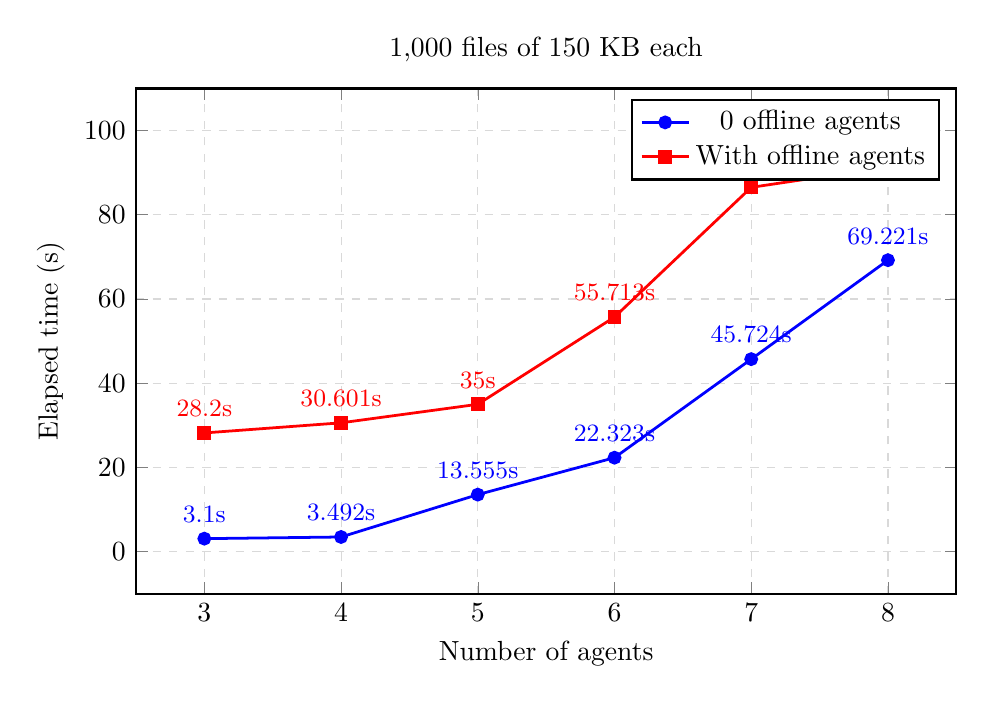
\begin{tikzpicture}
\begin{axis}[
    width=12cm, height=8cm,
    xlabel={Number of agents},
    ylabel={Elapsed time (s)},
    xmin=3, xmax=8,
    ymin=0, ymax=100,
    xtick={3,4,5,6,7,8},
    ytick={0,20,40,60,80,100},
    grid=major,
    grid style={dashed,gray!30},
    thick,
    title={1,000 files of 150~KB each},
    enlargelimits=0.1,
    clip=false,
    nodes near coords,
    every node near coord/.append style={font=\small, anchor=south, yshift=2pt},
    point meta=explicit symbolic
]

% Online agents
\addplot[color=blue, mark=*, line width=1pt] coordinates {
    (3,3.1) [3.1s]
    (4,3.492) [3.492s]
    (5,13.555) [13.555s]
    (6,22.323) [22.323s]
    (7,45.724) [45.724s]
    (8,69.221) [69.221s]
};

% Offline agents
\addplot[color=red, mark=square*, line width=1pt] coordinates {
    (3,28.2) [28.2s]
    (4,30.601) [30.601s]
    (5,35) [35s]
    (6,55.713) [55.713s]
    (7,86.510) [86.510s]
    (8,91.338) [91.338s]
};

\legend{0 offline agents, With offline agents}

\end{axis}
\end{tikzpicture}
\caption{Comparison of Corruption Check elapsed time with varying offline agents.}
\label{fig:test-3}
\end{figure}

\newpage
\paragraph{Test 4}
The fourth test demonstrates the system’s performance on a very large dataset consisting of 1,000,000 files of 3~B each, with only 3 agents online. The elapsed time, 217.4~s, shows that the system can handle extremely large numbers of files while maintaining reasonable check times. Figure~\ref{fig:test-4} displays the result.

\begin{figure}[!ht]
\centering
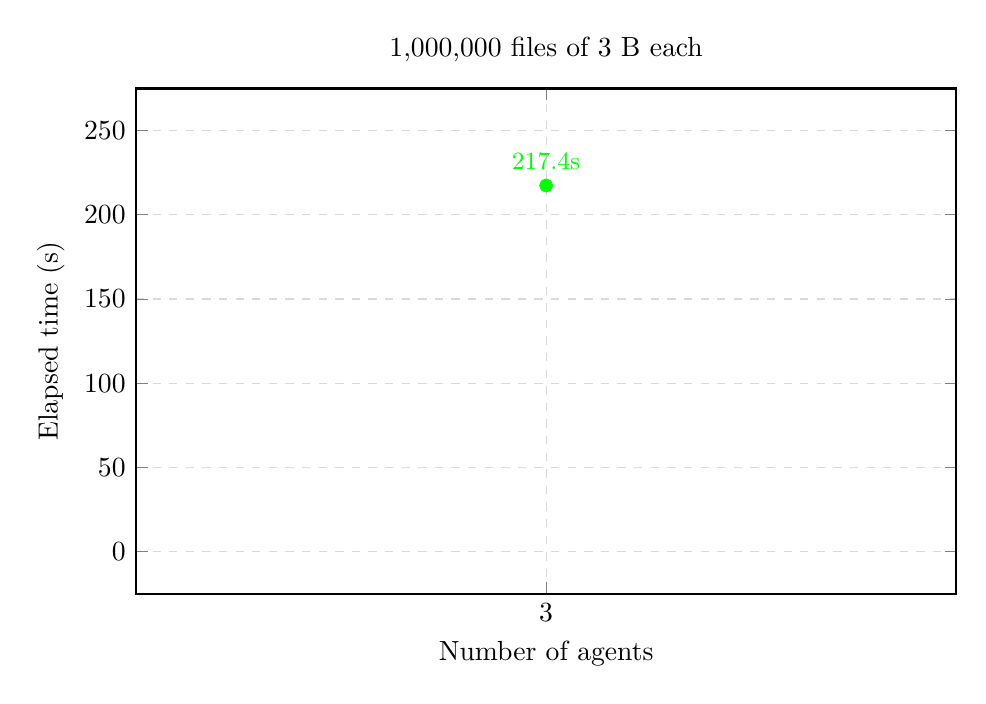
\begin{tikzpicture}
\begin{axis}[
    width=12cm, height=8cm,
    xlabel={Number of agents},
    ylabel={Elapsed time (s)},
    xmin=3, xmax=3,
    ymin=0, ymax=250,
    xtick={3},
    ytick={0,50,100,150,200,250},
    grid=major,
    grid style={dashed,gray!30},
    thick,
    title={1,000,000 files of 3~B each},
    enlargelimits=0.1,
    clip=false,
    nodes near coords,
    every node near coord/.append style={font=\small, anchor=south, yshift=2pt},
    point meta=explicit symbolic
]

\addplot[color=green, mark=*, line width=1pt] coordinates {
    (3,217.4) [217.4s]
};
\end{axis}
\end{tikzpicture}
\caption{Elapsed time for very large datasets.}
\label{fig:test-4}
\end{figure}
